\documentclass[a4paper,11pt]{article}
\usepackage{latexsym}
\usepackage[MeX]{polski}
\usepackage{polski}
\usepackage[utf8x]{inputenc}
\usepackage{graphicx}
\usepackage{mathtools}
\usepackage{pdfpages}
\usepackage{svg}
\usepackage{hyperref}
\usepackage[unicode]{hyperref}
\usepackage[polish]{babel}
\usepackage[ampersand]{easylist}




% Zdefiniowanie autora i~tytułu:
\author{Dawid Litwiński}
\title{lab}
\frenchspacing
\begin{document}
% Wstawienie autora i~tytułu do składu:
\maketitle
% Wstawienie spisu tre¶ci:
\tableofcontents
\newline
Do strony
\url{<inf.ug.edu.pl>}


\newpage

\section{matematyka}
\begin{matrix}
  a & b & c \\
  d & e & f \\
  g & h & i
 \end{matrix}
 
 \newline
 \newline
 \begin{equation}
\frac{
    \begin{array}[b]{r}
      \left( x_1 x_2 \right)\\
      \times \left( x'_1 x'_2 \right)
    \end{array}
  }{
    \left( y_1y_2y_3y_4 \right)
  }
\end{equation}

\section{grafika}
\DeclareGraphicsExtensions{.eps,.jpg}



\begin{figure}[!h]
% \includegraphics{obrazek.eps}



% \includepdf[pages={-}]{sloneczko.pdf}
% 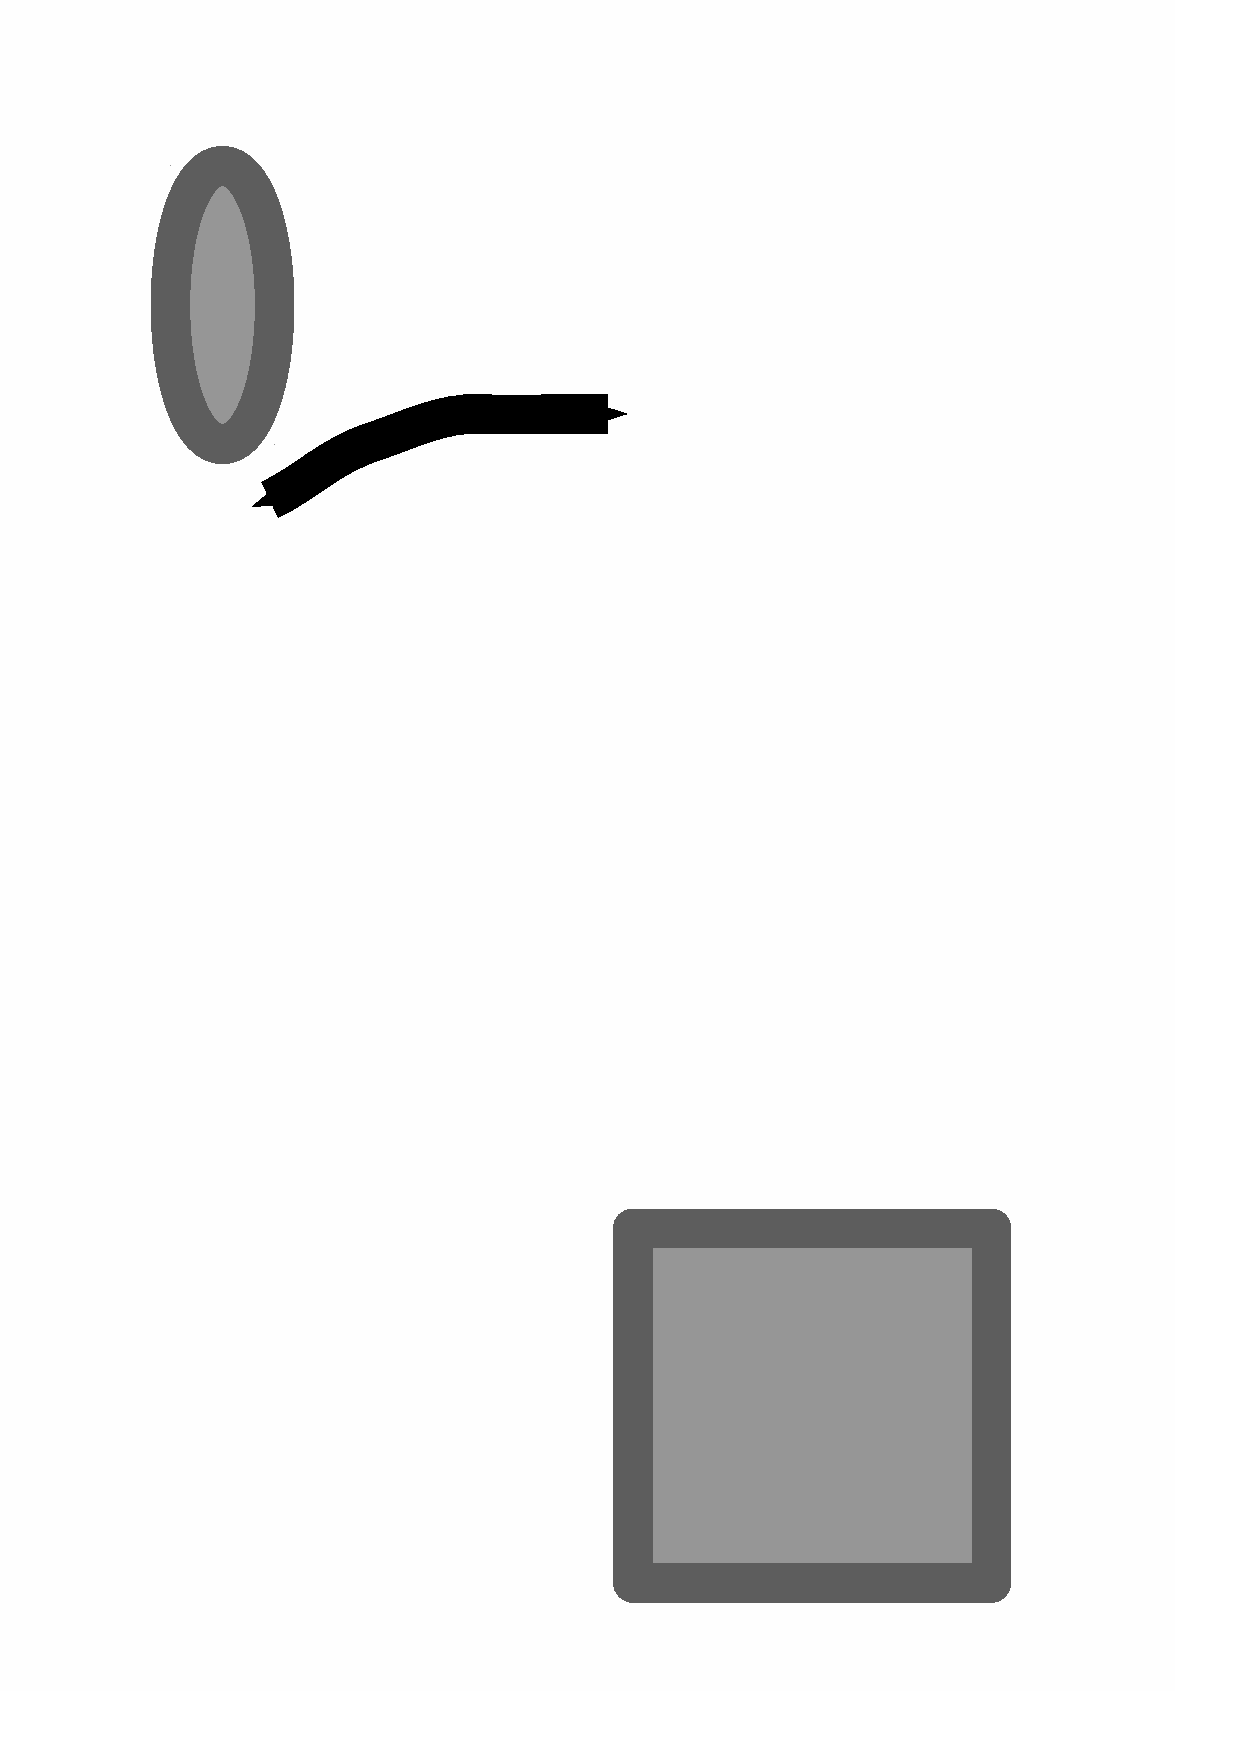
\includegraphics[scale=0.75]{wek.svg}}
\includegraphics[scale=0.05]{lit.jpg}
\end{figure}
\begin{figure}[!ht]
	\centering
		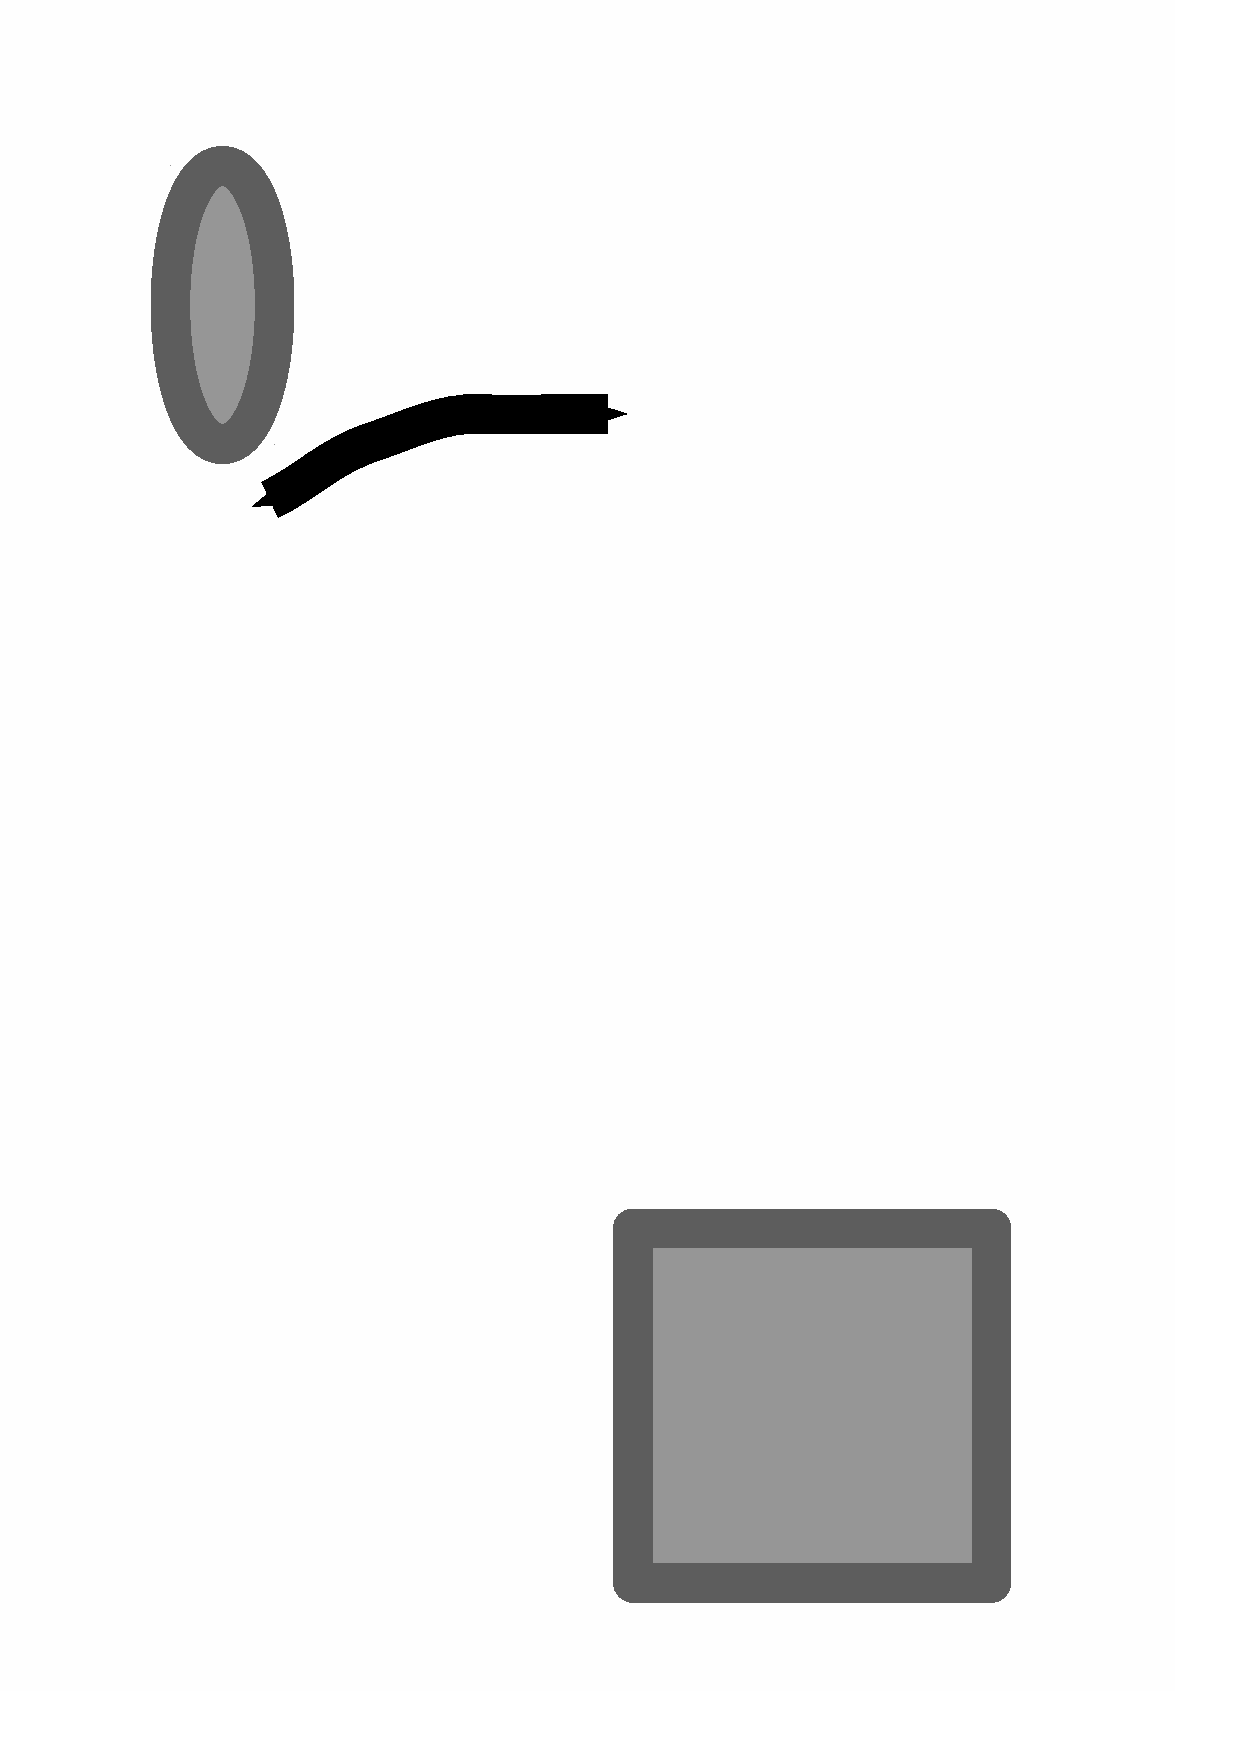
\includegraphics[width=0.40\textwidth]{wek.pdf}
	\caption{wektorowa \footnote{An example footnote.}}
	\label{fig:sloneczko}
\end{figure}




\section{Floats}
Floats are containers for things in a document that cannot be broken over a page. LaTeX by default recognizes "table" and "figure" floats, but you can define new ones of your own (see Custom floats below). Floats are there to deal with the problem of the object that won't fit on the present page, and to help when you really don't want the object here just now.

Floats are not part of the normal stream of text, but separate entities, positioned in a part of the page to themselves (top, middle, bottom, left, right, or wherever the designer specifies). They always have a caption describing them and they are always numbered so they can be referred to from elsewhere in the text. LaTeX automatically floats Tables and Figures, depending on how much space is left on the page at the point that they are processed. If there is not enough room on the current page, the float is moved to the top of the next page. This can be changed by moving the Table or Figure definition to an earlier or later point in the text, or by adjusting some of the parameters which control automatic floating.

Authors sometimes have many floats occurring in rapid succession, which raises the problem of how they are supposed to fit on the page and still leave room for text. In this case, LaTeX stacks them all up and prints them together if possible, or leaves them to the end of the chapter in protest. The skill is to space them out within your text so that they intrude neither on the thread of your argument or discussion, nor on the visual balance of the typeset pages.

\begin{description}
  \item[Pierwsze] \hfill \\
  teraz
  \item[Drugie] \hfill \\
  tam
  \item[nic] \hfill \\
  inne
\end{description}

\begin{enumerate}
  \item pierwsze
  \begin{enumerate}
    \item tu 1
    \item ter 2
  \end{enumerate}
  \item inn
\end{enumerate}


\begin{itemize}
  \item 1
  \item drugie
  \item wiecej \ldots
\end{itemize}

\begin{easylist}[checklist]
& glowny~:
&& pod.
&& inny pod.
\end{easylist}

\subsection{tabela}
\begin{tabular}{|7|2|}
  \hline
  Specifier & Permission\\
  \hline
  h & Place the float here, i.e., approximately at the same point it occurs \\
  \hline
    t & Position at the top of the page. \\
  \hline
    b & Position at the bottom of the page. \\
  \hline
    p & Put on a special page for floats only. \\
  \hline
    ! & Override internal parameters LaTeX uses for determining "good" float . \\
  \hline
    H & Places the float at precisely the location in the LaTeX code.. \\
  \hline
\end{tabular}

\begin{thebibliography}{9}

\bibitem{lamport94}
  Leslie Lamport,
  \emph{\LaTeX: a document preparation system}.
  Addison Wesley, Massachusetts,
  2nd edition,
  1994.

\end{thebibliography}
\end{document}
